\item The kinetic energy of a particle moving along a circle of radius \( R \) depends on the distance covered \( s \) as \( T = a s^2 \), where \( a \) is a constant. Find the force acting on the particle as a function of \( s \).
    \begin{center}
        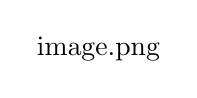
\begin{tikzpicture}
            \node at (0, 0) {{image.png}};
        \end{tikzpicture}
    \end{center}
\begin{solution}
    \begin{center}
        \begin{tikzpicture}
            \pic at (0, 0) {frame=3cm};
        \end{tikzpicture}
    \end{center}

    \begin{align*}
        \intertext{We have}
        T &= \frac{1}{2}mv^2 = as^2 \quad \text{or} \quad v^2 = \frac{2as^2}{m} \tag{1}
        \intertext{Differentiating Eq. (1) with respect to time}
        2vv_t &= \frac{4as}{m}v \quad \text{or} \quad v_t = \frac{2as}{m} \tag{2}
        \intertext{Hence net acceleration of the particle}
        w = \sqrt{w_t^2 + w_n^2} &= \sqrt{\left(\frac{2as}{m}\right)^2 + \left(\frac{2as^2}{mR}\right)^2} = \frac{2as}{m}\sqrt{1 + (s/R)^2}
        \intertext{Hence the sought, force $F = mw = 2as\sqrt{1 + (s/R)^2}$}
    \end{align*}
\end{solution}
